\section{Coordination Approaches}
Coordination approaches focus on how behavioral models interact one each other. They propose to specify the interaction between (heterogeneous) behavioral models in an additional model named \emph{model of coordination}. In this thesis, we adopt the wording of \emph{coordination} as being the explicit modeling of the interactions amongst behavioral models suitable to obtain the emerging system behavior. The coordination must be executable to enable the evaluation of the emerging behavior of the whole system. 

We categorize the coordination approaches into \emph{Model Coordination Approaches} and \emph{Language Coordination Approaches}. Model coordination approaches propose Coordination Languages~\cite{coordsignibib} and Architecture Description Languages (ADLs)~\cite{frameadlsbib} to specify the coordination between behavioral models. Languages Coordination approaches are Coordination Frameworks~\cite{ptoleframebib,modhelxbib} and Ad-hocs solutions~\cite{mascotbib,dinatale} that enable the automation of the coordination between models. To do so, they have captured the specification of a coordination pattern between languages into a tool or framework, \eg Ptolemy, ModHel'X. In the following, we first present model coordination approaches, and then, we continue with language coordination approaches.
\subsection{Model Coordination Approaches}
Model coordination approaches provide dedicated languages to specify the coordination between (heterogeneous) behavioral models (see Figure~\ref{fig:modelcoord}). We begin this subsection by presenting Coordination Languages, and then we continue with ADLs. 

\begin{figure}
	\begin{center}
		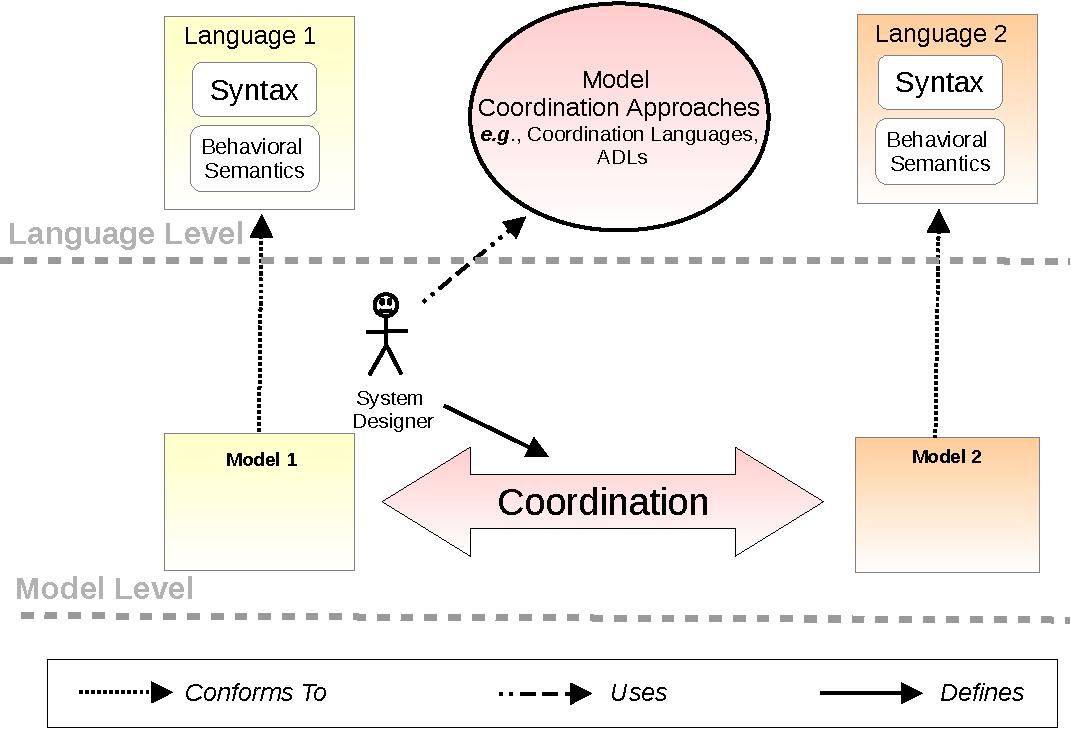
\includegraphics[width=.7\textwidth]{background/figs/coordmodel}
		\caption{Model Coordination Approaches Sketching}
		\label{fig:modelcoord}
	\end{center}
\end{figure}

Coordination Languages~\cite{coordsignibib} proposed a dedicated language to model the coordination between heterogeneous behavioral models. By relying on a coordination language, a system designer builds a coordination model to specify how behavioral models interact. Depending on the entities coordinated, approaches can be categorized into \emph{data-driven} or \emph{control-driven}. The former coordinates data among models whereas the latter coordinates events among models. Arbab at al.~\cite{whatdocoord} proposed another classification into \emph{endogenous} and \emph{exogenous} languages. Endogenous languages provide coordination primitives that must be incorporated within a model for its coordination. For instance, Linda~\cite{lindabib} provides a set of primitives like \emph{in()} or \emph{out()} to exchange data between models. These primitives must be added to a host language by using libraries. 

Exogenous coordination languages dealt with the complexity of model behaviors by treating models as black boxes encapsulated within the boundary of an interface. A model behavioral interface gives a partial representation of the model behavior therefore easing the coordination of behavioral models. The coordination is thus specified between elements of the interface. The notion of interface varies depending on the approach. For instance, in \emph{Opus}~\cite{Opus}, the interface is a list of methods provided by the model. Other approaches abstract away the non-relevant parts of the behavior of models as events~\cite{eventStructures} (also named signals in~\cite{lee1998framework}). These approaches focus on events and how they are related to each other through causal, timed or synchronization relationships. Following the same idea, \emph{control-driven} coordination languages rely on a model behavioral interface made of explicit events~\cite{esperbib,manifoldbib,coordinainterfacebib}. While in Esper~\cite{esperbib}, the interface is only a set of events acceptable by the model, some other approaches go further and also exhibit a part of the internal concurrency. This is the case of~\cite{coordinainterfacebib} where authors propose an interface that contains services and events, but also properties that express requirements on the behavior of the components. Such requirements act as a contract and can be checked during the coordination to ensure a correct behavior. The benefits of the use of events to coordinate the behavior of models are twofold:
\begin{itemize}	
	\item It gives support for control and timed coordination while remaining independent of the internal model implementation;
	\item It enables the coordination of models without any change to their implementation, thus ensuring a complete separation between the coordination and the computational concerns.
\end{itemize}

Concurrently with Coordination Languages, the \emph{software architecture} community has developed so-called Architecture Description languages (ADLs) to gain abstraction, structuring and reasoning capabilities~\cite{rapidebib,wrightbib,uniconbib,frameadlsbib,garlansoftarchbib}. An ADL usually specifies a system in terms of \emph{components} and interactions among those components. They enable a system designer to:
\begin{itemize}
	\item Clarify structural and semantics difference between a component and its interaction;
	\item Reuse and compose architectural elements;
	\item Identify/enforce commonly used patterns (\eg architectural styles).
\end{itemize}

Depending on the ADL, a \emph{Component} can be an encapsulation of some procedure, an encapsulation of an object file or a (formal) abstraction of its behavior. To externally characterize the components, ADLs rely on well identified \emph{Component Interfaces}. The interfaces are used by \emph{Connectors} whose behavior is specified by a \emph{glue}. Connectors can represent a large variety of interactions (\eg procedure call, event broadcast or database queries) and the glue can range from a simple function to complex protocols. 

Both coordination languages and ADLs make a separation between the specification of the component (\ie the computational aspects) and the assembly of these components (\ie the communication/coordination aspects). The latter is usually done by a system designer that has to deal with the architecture-level communication, which is expressed with different protocols. To abstract away these protocols and make them reusable, ADLs proposed connectors as types~\cite{frameadlsbib} that can be used on the shelf to specify domain specific interactions.

For example, Clara~\cite{clarabib} is an ADL dedicated to real time systems. It proposed built-in connector types like \emph{Rendez-vous}, \emph{Mutex} or \emph{Mailboxes}. A system designer can express the interactions by relying on these specific connectors that are relevant in his domain. This eases the task of a system designer, but also limits what can be used in the interaction. 

Other approaches introduced the notion of \emph{User Defined Type}~\cite{uniconbib,wrightbib,reobib} that enables a system designer to build connectors types for a specific domain. A connector type is defined by a set of \emph{roles} and a \emph{glue specification}. Roughly speaking, a role represents a formal parameter that is used to specify the glue which specifies how roles are coordinated. Some approaches express the glue in a formal language. For instance, in Wright~\cite{wrightbib}, the glue is specified in a variant of CSP~\cite{csphoarebib}, differently in Reo, it is specified by the composition of dedicated primitives~\cite{reobib}. The connector types are later on instantiated and the roles are bound to the actual interfaces of the instances of components. By expressing the glue in a formal language, the approaches can provide reasoning about the global system behavior. 

\begin{figure}
	\begin{center}
		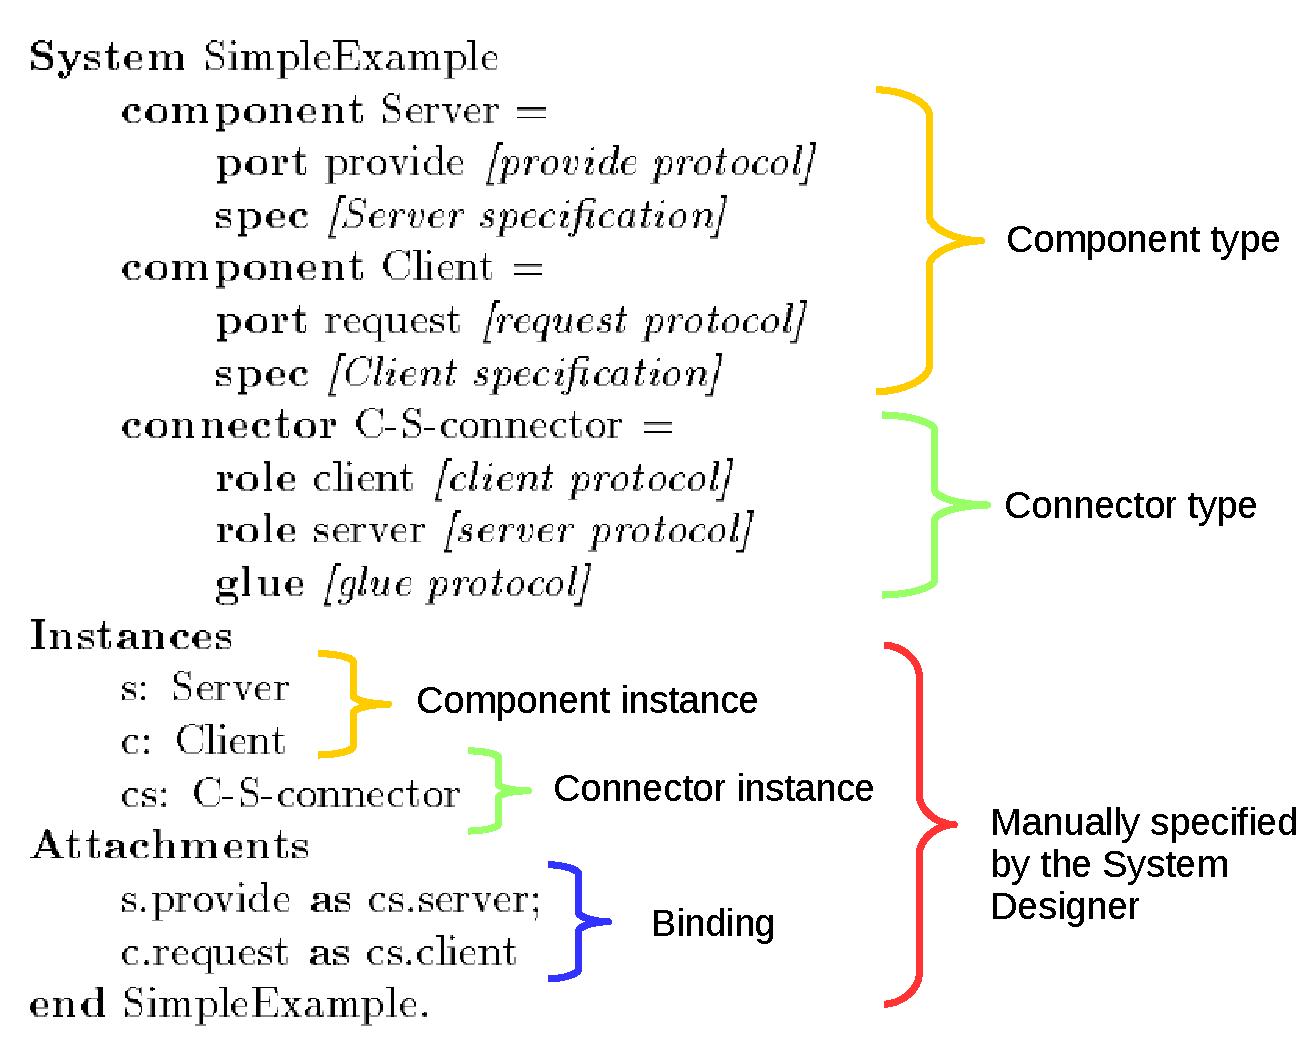
\includegraphics[width=0.7\textwidth]{background/figs/wrightspec}
		\caption{Specification of a Client-Server System in Wright~\cite{wrightbib}}
		\label{fig:wrightspec}
	\end{center}
\end{figure}

To illustrate the use of connector types, Figure~\ref{fig:wrightspec} shows a simple client-server system described in Wright~\cite{wrightbib}. The specification defines two component types named \emph{Client} and \emph{Server}, and one connector type named \emph{C-S-connector}. The C-S-connector has two roles (\emph{client} and \emph{server}) and a glue that describes how the activities of a client and a server roles are usually coordinated. The section \emph{Instances} describes a particular configuration by instantiating the corresponding component and connector types. The example describes a system where there is a single server (\emph{s}), a single client (\emph{c}) and a single connector (\emph{cs}). Then, the section \emph{Attachments} defines which component ports are attached to the connector roles.

In this subsection, we have presented approaches that make a clear separation between the specification of the component and the assembly of these components. While the first activity is usually done by a system engineer, the second one is usually done by a system designer. To ease the task of a system designer, ADLs community has successfully identified the need of connector types. In~\cite{wrightbib}, authors claimed that connector types enables to ``\emph{understand a general pattern of interaction that can occur many times in any given system}''. Thus, a system designer has only to instantiate and bind connector types as needed by its architecture. However, the major drawback of coordination languages and ADLs is that the coordination is specified between particular models. For example, in the case of ADLs, a system designer has to instantiate and bind connector types manually. Returning to the example of Figure~\ref{fig:wrightspec}, for each new client in the system, the system designer has to instantiate one component and one connector; then, he has to bind the component ports with the connector roles. With the increasing number and heterogeneity of the components, this task can quickly become difficult and error prone. We present in the next subsection approaches that automate the coordination between behavioral models by specifying coordination patterns between languages.

\subsection{Language Coordination Approaches}
Language Coordination Approaches have identified that the instantiation and binding of connector types can be a systematic activity the system designer repeats many times and may consequently be defined as a \emph{coordination pattern}. Such a pattern is based on the \emph{know-how} of the system designer and sometimes on naming or organizational conventions adopted by the models. In the following, we present approaches that have captured the specification of a \emph{behavioral coordination pattern} inside a tool/framework to automate the instantiation and binding of connector types. In these approaches, the coordination is specified between heterogeneous languages rather than between particular models. We begin this subsection by presenting ad-hoc solutions~\cite{mascotbib, dinatale} which fix the language that they coordinate. We continue with more systematic approaches named Coordination Frameworks~\cite{modhelxbib,ptoleframebib}.


MASCOT~\cite{mascotbib} is an approach focused on the integration of Matlab~\cite{matlabbib} and SDL~\cite{sdlbib}. Whereas SDL is a language suitable for control systems modeling, Matlab is better for modeling dataflow aspects of a system. These languages are rather different: while SDL processes operate on events, represented by simple signals, Matlab processes operate on vectors, represented by vectorized signals. Authors proposed to automate the synchronization of control signals from SDL with data signals from Matlab. To do so, the approach deals with the integration of the timing and synchronization concepts from both languages by proposing two synchronization modes: \emph{head synchronization} and \emph{tail synchronization}. In the head synchronization, when a model in matlab receives a frame \emph{a1}, it immediately transforms \emph{a1} into \emph{b1} (dataflow network model). Any control signal from SDL that occurs during the transformation of \emph{a1} to \emph{b1} cannot influence its value. Then, the head synchronization mode ensures that the occurrence of the control signal is taken into account when the next frame is processed. In the tail synchronization, when a model in Matlab receives a control signal from SDL, the signal is collected until it cease to occur, then, it is translated to a vector and passed to the Matlab model. The modes of synchronization ensure the communication between Matlab and SDL by relying on the knowledge about the semantics of the languages. In addition, the approach gives a set of guidelines to help the choice between the two proposed synchronization. Once the synchronization policy is defined, the approach enables the co-simulation of a SDL model and a Matlab model. A process in the SDL specification that is specified in Matlab contains a wrapper that interfaces between the SDL simulator and the Matlab engine. A SDL wrapper is made of a set methods that enable the SDL engine to control the behavior of the data signals in Matlab. To do so, the approach relies on the name of signals in SDL specification to communicate with the signals in Matlab. Thus, the approach forces a naming convention between signals in both domains. The approach has identified and specified a coordination pattern between Matlab and SDL by providing two mechanisms to coordinate signals from both domains. In addition, it provides some guidelines to help the choice between the two mechanism. The current implementation, however, partially automates the coordination since the user has to specify what synchronization mechanism is used.

\begin{figure}[ht!]
	\begin{center}
		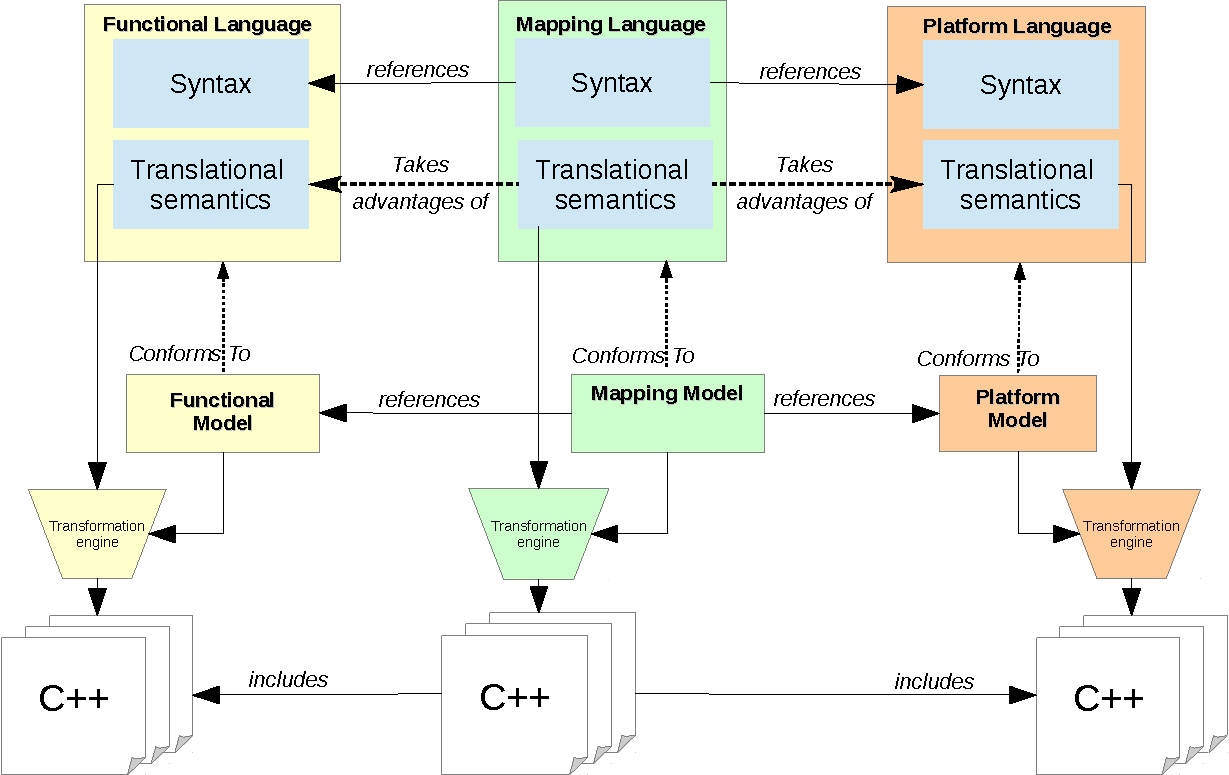
\includegraphics[width=0.8\textwidth]{background/figs/diNatale}
		\caption{High Level View of the Approach Proposed by Di Natale et al. in~\cite{dinatale}}
		\label{fig:diNatale}
	\end{center}
\end{figure}

In~\cite{dinatale} (see Figure~\ref{fig:diNatale}), authors dealt with the integration of a language to describe the functional aspects of a system with a language to describe the deployment platform of the system. They proposed to integrate these languages by relying on a dedicated mapping language. The mapping language syntax references syntactic elements from both the functional and the platform language to map the functions on specific computational resources from the platform. For instance, the $SWdeployment$ concept from the mapping model, references the $Task$ concept from the functional model and the $CPU$ concept from the platform model. Based on the mapping model, the approach generates the code of the communication between the code of the functional and the code of the platform models. The semantics of both the functional and the platform languages are defined by a translational approach into C++ code. The translational semantics of the mapping language takes advantages of some knowledges about the translational semantics of the other languages. For instance, for each subsystem in the functional language, the approach takes advantages of the knowledge that a class is generated with a name like: \emph{SubsystemName}\texttt{ModelClass}. It also takes advantage from the knowledge that the generated class has a \texttt{step} operation used for the runtime evaluation of the block outputs given its inputs and its internal state. 

To express a coordination pattern between a functional and a platform language, the approach proposed a set of connectors to specify the mapping of a functional model to a platform model. From the mapping model, the approach generates the communication code between a functional and a platform model. In this sense, the approach is similar to others ADLs that propose a set of built-in connectors. The approach partially automates the coordination between models since a system designer has to instantiate the connectors.  

\begin{figure}[ht!]
	\begin{center}
		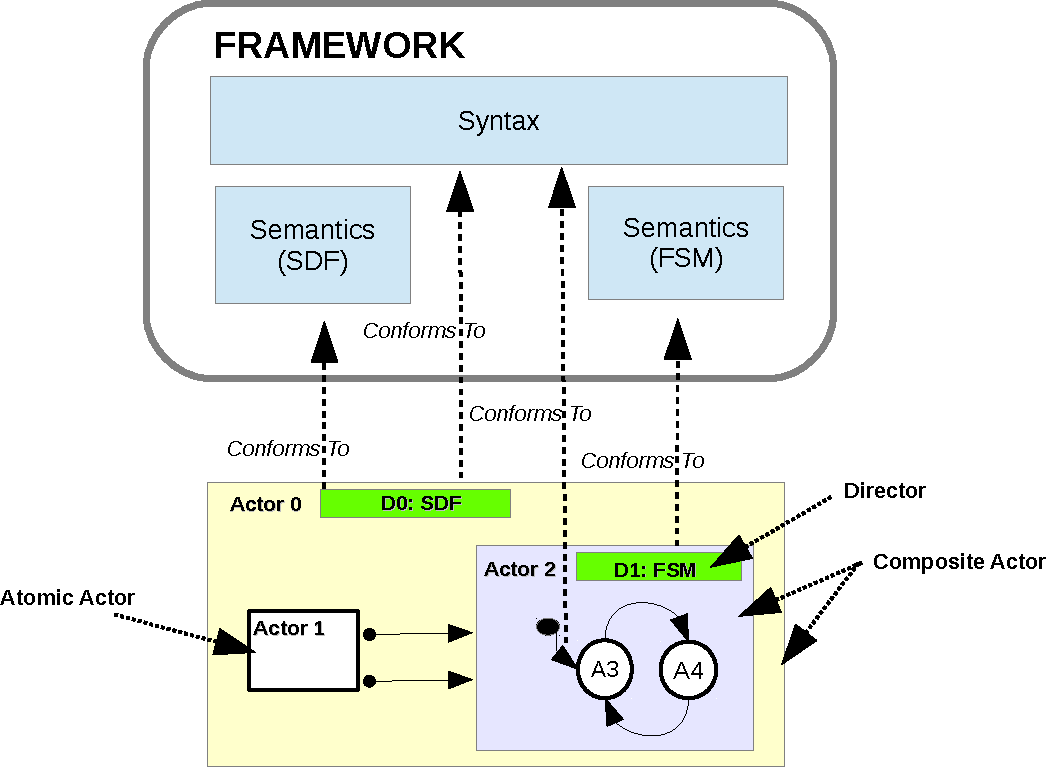
\includegraphics[width=0.8\textwidth]{background/figs/ptolemyfig}
		\caption{High Level View of Ptolemy~\cite{giraultbib}}
		\label{fig:ptolemyfig}
	\end{center}
\end{figure}

While the previous approaches are ad-hoc solutions for two particular languages, Ptolemy~\cite{ptoleframebib} and ModHel'X~\cite{modhelxbib} are systematic approaches to coordinate models that conform to heterogeneous languages. These approaches rely on a framework in which the syntax of models is described by actors and the semantics is given by a Model of Computation (MoC). Actors can be atomic (\eg \emph{Actor 1} in Figure~\ref{fig:ptolemyfig}) or composite (\eg \emph{Actor 0} and \emph{Actor 2} in Figure~\ref{fig:ptolemyfig}), \ie made of internal, connected, actors. Each composite actor is associated with a model of computation that defines a \emph{Domain}. A domain specifies both the communication semantics and the execution order among internal actors. A domain is implemented by a \emph{Director}. For instance, in Figure~\ref{fig:ptolemyfig}, \emph{Actor 0} has the director \emph{D0}, which implements a SDF (Synchronous Dataflow) domain, and the \emph{Actor 2} has the director \emph{D1}, which implements a FSM (Finite State Machine) domain. In this approach, actors, both atomic and composite, are executable. In a composite actor, the execution order of internal actors is controlled by a director. In the example of Figure~\ref{fig:ptolemyfig}, the director \emph{D0} controls the execution of the \emph{Actor 1} and \emph{Actor 2} and director \emph{D1} controls the execution of \emph{A3} and \emph{A4} whenever \emph{Actor 2} is executed. In this sense, the execution of composite actors is strictly hierarchical. The behavior of actors is represented by a generic interface that contains a set of methods, \eg fire(). The MoC implemented by the director of a composite actor specifies when the methods in the interface of internal actors are invoked. For instance, when an actor is fired, the director associated with a composite actor fires the internal actors. 

In conclusion, based on a fixed syntax and a generic interface, these approaches achieved to capture a hierarchical coordination pattern into a framework. For the syntactic aspects of the pattern, the framework provides composite actors. Then, for the semantical aspects, the framework encodes the necessary glue between interfaces of composite actors and internal actors to coordinate their execution. This results in a hierarchical heterogeneous model in which the execution of actors is strictly hierarchical.

In this subsection, we have presented approaches that captured the specification of a coordination pattern between languages. Such specification is defined at language level and captures a systematic way to coordinate behavioral models. By specifying the coordination at language level, these approaches have achieved to automate the coordination between models. In the next subsection, we discuss about the previous reviewed approaches.   

\subsection{Discussion}
In this section, we have studied approaches to coordinate the behavior of models. While model coordination approaches proposed dedicated languages to build a model of coordination, Language coordination approaches proposed frameworks/tools that automate the coordination between models by specifying a coordination pattern between languages. 

Model Coordination approaches provide dedicated languages, \ie Coordination Languages, ADLs, to specify the coordination between particular models. Such a model of coordination specifies how the behavioral models interact. The main benefit of these approaches is that the global behavior is explicit and amenable for reasoning (for instance for Verification and Validation activities). Furthermore, they propose languages close to system designer domain. For example, ADLs provide types in order to define domain-specific connectors. ADLs have successfully identified connectors type, however, a system designer has still to instantiate the required type of connectors when needed; he has to manually instantiate them by relying on his know-how. In a complex system, such a task can quickly become tedious and error prone. Furthermore, if one of the model changes, the model of coordination must also be changed. By relying on Coordination Languages and ADLs, a system designer only captures the solution for one single problem but he does not specify a systematic way to coordinate models. 

Coordination frameworks achieved to capture the know-how of a system designer by specifying coordination patterns. Such specification defined at the language level allows for synthesis the coordination between heterogeneous behavioral models. %However, these approaches still need a system designer to, for instance, choose the synchronization mechanism~\cite{mascotbib}, or instantiate the connectors~\cite{dinatale}.   

By embedding the coordination pattern inside a tool, these approaches have two major drawbacks:
\begin{itemize}
	\item 1) Validation and verification activities are limited since the coordination is encoded by using a general purpose language (\eg Java in Ptolemy and ModHel'X);
	\item 2) The system designer cannot change the proposed coordination without altering the core of the tool.  
\end{itemize}
Regarding to first point, some coordination languages and ADLs already tackled this problem by using a formal language to express the coordination (\eg CSP in Wright). This provides for verification and validation support for the coordinated system

Concerning the second point, for complex systems, the system designer may need to capture several coordination patterns and potentially combine them. However, current coordination frameworks can only support such a variation by modifying the framework itself. The coordination model is mixed with the functional model, which makes it very tricky to modify one without risking altering the other.



%To be executable, each DSML defines a behavioral semantics. The specification of the behavior semantics of a DSML varies from natural language to the use of a formal language. In any case, the developing of complex applications relies on heterogeneous DSMLs thus resulting in heterogeneous behavioral models. 

%Model coordination is a modeling approach to integrate the behavior of models. It proposes to specify the interaction between heterogeneous behavioral models by relying on a \emph{model of coordination}. According to \cite{coordsignibib}, ``\textit{Coordination is the process of building programs by gluing together active pieces}''. In this thesis, we adopt the word \emph{coordination} as being the explicit modeling of the interactions amongst behavioral models to obtain the emerging system behavior. In this sense, the coordination must be executable to enable the evaluation of the emerging behavior of the whole system. 

%The goal of coordination is the integration of behavioral models. Clavreul~\cite{clavreulmodelcompo} has identified two commons issues in the integration of systems: 
%\begin{itemize}
%	\item The models are developed independently by relying on different technologies;
%	\item It is very often forbidden to modify existing systems to implement the integration.   
%\end{itemize}
%In this context, Coordination approaches propose to define the interactions between models separately from the computation. As a result, the existing models are not changed and the coordination only constrains theirs behaviors. 

%In this section, we present an overview of approaches that coordinate the behavior of models and languages. We categorize them into \emph{Coordination Languages and Architecture Description Languages}, and \emph{Coordination Frameworks}. The former enables a system designer to model the coordination between models whereas the latter provides a tool to automate the coordination of heterogeneous models by specifying the coordination between heterogeneous languages.

%Coordination Languages have been proposed by Carriero et al.~\cite{coordsignibib} to model the coordination between heterogeneous behavioral models. Depending on the entities coordinated, approaches can be categorized into \emph{data-driven} or \emph{control-driven}. The former coordinates data among models whereas the latter coordinates events among models. Arbab at al.~\cite{whatdocoord} propose another classification into \emph{endogenous} and \emph{exogenous} languages. Endogenous languages provide coordination primitives that must be incorporated within a model for its coordination. For instance, Linda~\cite{lindabib} provides a set of primitives like \emph{in()} or \emph{out()} to exchange data between models. These primitives must be added to a host language by using libraries. 


%Some coordination languages deal with the complexity of model behaviors by treating models as black boxes encapsulated within the boundary of an interface. A model behavioral interface gives a partial representation of the model behavior therefore easing the coordination of behavioral models. However, it is not uniquely defined and may vary depending on approaches. For instance, in \emph{Opus}~\cite{Opus}, the interface is a list of methods provided by the model. Other approaches abstract away the non-relevant parts of the behavior of models as events~\cite{eventStructures} (also named signals in~\cite{lee1998framework}). These approaches focus on events and how they are related to each other through causal, timed or synchronization relationships. Following the same idea, \emph{control-driven} coordination languages rely on a model behavioral interface made of explicit events~\cite{rapide,esperbib,coordinainterfacebib}. While in Rapide~\cite{rapide}, the interface is only a set of events acceptable by the model, some other approaches go further and also exhibit a part of the internal concurrency. This is the case of~\cite{coordinainterfacebib} where authors propose an interface that contains services and events, but also properties that express requirements on the behavior of the components. Such requirements act as a contract and can be checked during the coordination to ensure a correct behavior. In these approaches, the model behavioral interface provides information to coordinate the behavior of a model.



%Conversely, exogenous coordination languages deal with the complexity of model behaviors by treating models as black boxes encapsulated within the boundary of an interface. A model behavioral interface gives a partial representation of the model behavior therefore easing the coordination of behavioral models. The coordination is thus specified between elements of the interface. The notion of interface varies depending on the approach. For instance, in \emph{Opus}~\cite{Opus}, the interface is a list of methods provided by the model. Other approaches abstract away the non-relevant parts of the behavior of models as events~\cite{eventStructures} (also named signals in~\cite{lee1998framework}). These approaches focus on events and how they are related to each other through causal, timed or synchronization relationships. Following the same idea, \emph{control-driven} coordination languages rely on a model behavioral interface made of explicit events~\cite{esperbib,manifoldbib,coordinainterfacebib}. While in Esper~\cite{esperbib}, the interface is only a set of events acceptable by the model, some other approaches go further and also exhibit a part of the internal concurrency. This is the case of~\cite{coordinainterfacebib} where authors propose an interface that contains services and events, but also properties that express requirements on the behavior of the components. Such requirements act as a contract and can be checked during the coordination to ensure a correct behavior. The benefits of event-driven coordination languages are twofold:
%\begin{itemize}
%	\item They give support for control and timed coordination while remaining independent of the internal model implementation;
%	\item They coordinate models without any change to their implementation, thus ensuring a complete separation between the coordination and the computational concerns.
%\end{itemize} 


%\todo{ADLs are based on the idea to keep computation and coordination as different concerns. They are control drive coordination languages (exogenenous). In this aproaches, the concepts of interfaces and connector become very important}

%Concurrently, the \emph{software architecture} community has developed so-called Architecture Description languages (ADL) to gain abstraction, structuring and reasoning capabilities~\cite{rapidebib,wrightbib,uniconbib,frameadlsbib,garlansoftarchbib}. An ADL usually specifies a system in terms of \emph{components} and interactions among those components. They enable a system designer to:
%\begin{itemize}
%	\item Clarify structural and semantics differences between components and interactions;
%	\item Reuse and compose architectural elements;
%	\item Identify/enforce commonly used patterns (\eg architectural styles).
%\end{itemize}
%Depending on the ADL, a \emph{Component} can for instance be an encapsulation of some procedure, an encapsulation of an object file or a (formal) abstraction of its behavior. To externally characterize the components, ADLs rely on well identified \emph{Component Interfaces}. The interfaces are used by \emph{Connectors} whose behavior is specified by a \emph{glue}. Connectors can represent a large variety of interactions (\eg procedure call, event broadcast or database queries) and the glue can range from a simple function to complex protocols. 

%Both coordination languages and ADLs make a clear separation between two design activities: the specification of the component (\ie the computational aspects) and the assembly of these components (\ie the communication/coordination aspects). While the first activity is usually done by a software engineer, the second one is done by a system designer. The latter has to deal with the architecture-level communication as expressed with complex protocols. To abstract away these protocols and make them reusable, ADLs propose on-the-shelves connectors as types~\cite{frameadlsbib} to specify domain specific interactions.

%For example, Clara~\cite{clarabib} is an ADL dedicated to real time systems. It proposes built-in connector types like \emph{Rendez-vous}, \emph{Mutex} or \emph{Mailboxes}. This helps the task of a system designer by providing relevant domain specific connectors. However, this also limits what can appear in the interactions. 

%Other approaches have introduced the notion of \emph{user defined type}~\cite{uniconbib,wrightbib,reobib} that enables a system designer to build connectors for an specific domain. A connector type is defined by a set of \emph{roles} and a \emph{glue specification}. Roughly speaking, a role represents a formal parameter that is used to specify the glue. The glue is based on a formal language to specify how roles are coordinated. For instance, in Wright~\cite{wrightbib}, the glue is specified in a variant of CSP~\cite{csphoarebib}, whereas in Reo it is specified by the composition of dedicated primitives~\cite{reobib}. The connector types are later on instantiated and the roles are bound to the actual interfaces of the component instances. 
%\\

%To illustrate how a system designer can define a set of domain specific connector types, Figure~\ref{fig:wrightspec} shows a simple client-server system described in Wright~\cite{wrightbib}. The specification defines two component types named \emph{Client} and \emph{Server}, and one connector type named \emph{C-S-connector}. The C-S-connector has two roles (\emph{client} and \emph{server}) and a glue that describes how the activities of the client and server roles are coordinated. The section \emph{Instances} describes a particular configuration by instantiating the corresponding components and connectors. The example describes a system where there is a single server (\emph{s}), a single client (\emph{c}) and a single connector (\emph{cs}). Then, the section \emph{Attachments} defines which component ports are attached to the connector roles. ADLs have successfully identified the need of connector types in order to ease the task of a system designer. In~\cite{wrightbib}, authors claim that connector types enables to ``\emph{understand a general pattern of interaction that can occur many times in any given system}''. Thus, a system designer has only to instantiate and bind connector types as needed by its architecture. 

%The major drawback of coordination languages and ADLs is that the specification of the coordination is between particular models. For example, in the case of ADLs, a system designer has to instantiate and bind connector types manually. Returning to the example of Figure~\ref{fig:wrightspec}, for each server and client in the system, the system designer has to instantiate two components and one connector. Then, he has to bind the component ports with the connector roles. With the increasing number and heterogeneity of the components, this task can quickly become difficult and error prone.

%\emph{Coordination Frameworks} have identified that the instantiation and binding of connector types can be a systematic activity that the system designer repeats many times and can consequently be defined as a pattern. Such a pattern is based on the \emph{know-how} of the system designer and sometimes on naming or organizational conventions adopted by the models. Thus, they have captured the specification of a \emph{behavioral coordination pattern} inside a tool/framework to automate the instantiation and binding of connector types. In these approaches, the coordination is specified between heterogeneous languages rather than among particular models. 

% maltab and sdl has a sintax but also a semantics coompletly different. 
% matlab is data flow (sdf) y sdl (control flow or fsm)
% matlab vectores de datos, sdl events. 
% implementa como sincronizar eventos con datos

%For example, MASCOT~\cite{mascotbib} is an approach focusing on the integration of Matlab~\cite{matlabbib} and SDL~\cite{sdlbib}. Whereas SDL is a language suitable for control systems modeling, Matlab is better for modeling dataflow aspects of a system. However, these languages are very different, while SDL processes operate on events, represented by simple signals, Matlab processes operate on vectors, represented by vectorized signals. Thus, authors propose to automate the synchronization of control signals from SDL with data signals from Matlab. These signals can either be notification signals or message signals. Notification signals do not carry a value and are used to notify a process when an event occurs. Message signals carry a value and are used to indicate a change of some variable or parameter. The approach deals with the integration of the timing and synchronization concepts from both languages by proposing two synchronization modes: head synchronization and tail synchronization. These mechanisms take advantages of the knowledge about the semantics of the languages. For instance, in the head synchronization, when a model in matlab receives a frame \emph{a1}, it immediately transforms \emph{a1} into \emph{b1} (dataflow network model). Any control signal from SDL that occurs during the transformation of \emph{a1} to \emph{b1} cannot influence its value. Then, the head synchronization mode ensures that the occurrence of the control signal is taken into account when the next frame is processed. In the tail synchronization, when a model in Matlab receives a control signal from SDL, the signal is collected until it ceases to occur, then, it is translated into a vector and passed over to the Matlab model. The synchronization modes ensure the communication between Matlab and SDL. In addition, the approach gives a set of guidelines to aid the system designer choose between the two synchronization policies proposed. Once the synchronization policy defined, the approach enables the co-simulation of a SDL model and a Matlab model. The implementation is based on SDL wrappers. A process in the SDL specification that is specified in Matlab contains a wrapper that interfaces between the SDL simulator and the Matlab engine. A SDL wrapper is made of a set methods that enable the SDL engine to control the behavior of the data signals in Matlab. To do so, the approach relies on the name of signals in SDL specification to communicate with the signals in Matlab. The approach thus forces the system designer to follow a naming convention between signals in both domains. Although the current implementation partially automates the coordination of signals from both domains, the approach has identified and captured a coordination pattern between a control-flow language and a data-flow language by relying on some knowledge about its syntax and semantics.

%In~\cite{dinatale} (see Fig.\ref{fig:diNatale}), authors deal with the integration of two languages. One language to describe the functional aspects and another language to describe the platform. The integration relies on a dedicated mapping language whose syntax references syntactic elements from both the functional and platform languages. 
%For instance, the $SWdeployment$ concept from the mapping model, references the $Task$ concept from the functional model and the $CPU$ concept from the platform model. Based on the mapping model, the approach generates the code of the communication between the functional and platform models. The semantics of both the functional and the platform languages is defined by an translational approach into C++ code. The translational semantics of the mapping language takes advantages of some knowledges about the translational semantics of the other languages. For instance, for each subsystem in the functional language, authors know that a class is generated with name \emph{SubsystemName}\texttt{ModelClass}. They also know that the class has a \texttt{step} operation for the runtime evaluation of the block outputs given the inputs and the state. Thus, from a mapping model, the approach can generate the code to communicate between the functional and platform models. The approach proposes a set of connectors that the system designer has to instantiate in the mapping model. In this sense, it is similar to ADLs that propose a set of built-in connectors. However, different from ADLs relying on connectors types to link concepts from the syntax of languages. In particular,  connector types capture some knowledge of a system designer that performs the mapping of a functional model to a platform model. 

%The semantics of both the functional and the platform language is defined by an translational approach into C++ code. 

%This approach has achived to: 1) propose a dedicated language to explicitly relate concepts from both languages. Such a language contains as a built-in connector types that the developer can instantiate. 2) From such connectors, a generative approach enables to generate the comunication code in C++. 



%A first interesting aspect of this approach comes from the possibility, by creating a dedicated language, to reuse existing languages, and based on a mapping model to automatically generate the glue between the implementation of the models (in this case encoded in C++). 

%The mapping language syntax references syntactic elements from both the functional and the platform language. For instance, the $SWdeployment$ concept from the mapping model, references the $Task$ concept from the functional model and the $CPU$ concept from the platform model. 


%The translational semantics of the mapping language takes advantages of some knowledges about the translational semantics of the other languages. For instance, for each subsystem in the functional language, authors know that a class is generated with name \emph{SubsystemName}\texttt{ModelClass}. They also know that the class has a \texttt{step} operation for the runtime evaluation of the block outputs given the inputs and the state. 

%In other words, authors have a partial but sufficient knowledge of the translational semantics of both the functional and the platform language. 

%Finally, based on this knowledge, they encode in the translational semantics the glue to generate according to the actual mapping in the mapping model. 
 
 %While the previous approaches are ad-hoc solutions for two particular languages, Ptolemy~\cite{ptoleframebib} and ModHel'X~\cite{modhelxbib} are systematic approaches to coordinate models that conform to a set of predefined languages. These approaches rely on frameworks in which the syntax of models is described by actors and the semantics is given by a Model of Computation (MoC). Actors can be atomic (\eg \emph{Actor 1} in Figure~\ref{fig:ptolemyfig}) or composite (\eg \emph{Actor 0} and \emph{Actor 2} in Figure~\ref{fig:ptolemyfig}), \ie made of internal actors. Each composite actor is associated with a model of computation that defines its \emph{Domain}. A domain specifies the communication semantics and the execution order among internal actors. A domain is implemented by a \emph{Director}. For instance, in Figure~\ref{fig:ptolemyfig}, \emph{Actor 0} follows director \emph{D0}, which behaves according to the semantics of SDF and \emph{Actor 2} follows director \emph{D1} that implements the semantics of FSM. In this approach, actors, both atomic and composite, are executable. In composite actors, the execution order of internal actors is controlled by a director. In the example of Figure~\ref{fig:ptolemyfig}, director \emph{D0} controls the execution of \emph{Actor 1} and \emph{Actor 2} and director \emph{D1} controls the execution of \emph{A3} and \emph{A4} whenever \emph{Actor 2} is executed. In this sense, the execution of composite actors is strictly hierarchical. The behavior of actors is represented by a generic interface that contains a set of methods, \eg fire(). The MoC implemented by the director of a composite actor specifies when the methods in the interface of internal actors are invoked. For instance, when a composite actor is fired, the director associated with the composite actor fires the actors of the contained model. Based on a fixed syntax and a generic interface, these approaches have achieved to capture a hierarchical coordination pattern into a framework. The framework provides a dedicated syntax to specified the pattern, \ie composite actors, and encodes the necessary glue between interfaces to coordinate their execution. 
%\\
  
%\subsection{Discussion}
%Coordination languages and ADLs enable the system designer to define one or more models of coordination to specify how behavioral models interact. The main benefit of these approaches is that the global behavior is explicit and amenable for reasoning (for instance for Verification and Validation activities). Furthermore, they propose languages close to system designer domain. For example, ADLs provide types in order to define domain-specific connectors.  

%These approaches have successfully identified connector types, however, a system designer has still to specify when a type of connectors is used. He has to manually instantiate them by relying on his know-how. In a complex system, such a task can quickly become tedious and error prone. Furthermore, if one of the model changes, the model of coordination must also be changed. By relying on Coordination Languages and ADLS, a system designer only captures the solution for one single problem but he is not able to specify a systematic way to coordinate models. 

%Conversely, Coordination frameworks have achieved to capture the know-how of a system designer by specifying coordination patterns. Such specification at language level allows automating the coordination between behavioral models. However, they embed the coordination pattern inside a tool. This has two major drawbacks:
%\begin{itemize}
%	\item 1) Validation and verification activities are limited since the coordination is encoded by using a general purpose language (\eg Java in Ptolemy and ModHel'X);
%	\item 2) The system designer cannot change the proposed coordination without altering the core of the tool. 
%\end{itemize} 
%Regarding to the first point, coordination languages and ADLs have already tackled this problem by using a formal language to express the coordination (\eg CSP in Wright). This provides for verification and validation support for the coordinated system. Recent work in that direction~\cite{semanticadaptccsl} uses the Clock Constraint Specification Language(CCSL)L~\cite{ccslbib} to specify the semantic adaption in ModHel'X. 

%Concerning the second point, for complex systems, the system designer may need to capture several coordination patterns and potentially combine them. However, current coordination frameworks can only support such a variation by modifying the framework itself. The coordination model is mixed with the functional model, which makes it very tricky to modify one without risking altering the other.

%To summarize, two main achievements of coordination approaches are:
%\begin{itemize}
%	\item To capture the interactions between behavioral models in an explicit and formal way; 
%	\item To leverage on the system designer know-how by capturing coordination patterns. 
%\end{itemize}